\section{Muons} \label{sec:objects:muons}

As muons traverse the entire detector they leave a track of charge depoosits in
the Inner Detector (ID) and Muon Spectrometer (MS) which is then reconstructed to
represent the path of the muon \cite{Aad:2016jkr}. This results in four
different muon types dependant upon which subdetectors were used in the
reconstruction:

\begin{enumerate}
  \item Combined (CB) muons: First the charged track is reconstructed independently in the ID and MS.  Then a global refit combines the hits from both subdetectors. This global fit may add or subtract MS hits from the track to achieve the best fit quality.
  \item Segment-tagged (ST) muons: A track is developed in the ID and then extrapolated to the MS.  If this extrapolation finds at least one local track segment in the MDT or CSC it is labeled a muon.  This is generally used for low $p_{T}$ muons which may only traverse one layer of the MS.
  \item Calorimeter-tagged (CT) muons: Here a track formed in the ID is labeled a muon if it can be associated with a calorimeter deposit consisent with a minimum-ionizing particle.  This is the least pure muon type but allows for reconstruction of muons that pass through the partially instrumented region of the MS.
  \item Extrapolated (ME) muons: These muons are reconstructed using only MS track information and the loose requirement that the hits are compatible with a trajectory originating from the interaction point.  This type is useful for extending the muon acceptance into the region not covered by the ID.
\end{enumerate}

After the muon type is determined we categorize the quality of the muon by
requiring a specific number of hits in each subcomponent.  These quality requirements are provided to address the specific needs of different physics anlysis. The four muon quality levels are defined:

\begin{enumerate}
  \item[\texttt{loose}] The lowest quality is designed to maximize the reconstruction efficiency for muons allowing all muon types to be used.  This is primarly useful for analysis resulting in multi-leptonic final states such as $H \rightarrow 4\ell$.
  \item[\texttt{medium}] Designed to minimize the systematic uncertainties associated with muon reconstruction and calibration.  Only CB and ME tracks are used requiring at least 3 CB track hits and at least 3 ME layers.  This is the default quality selection in ATLAS and the one used for muons in this thesis.
  \item[\texttt{tight}] This selection maximizes the purity of muons but reduces the reconstruction efficiency. Here only CB muons with at least 2 layers of the MS that also satisfy the \texttt{medium} selection requirements are allowed.
  \item[\texttt{high-$p_{T}$}] Designed to maximize the momentum resolution for tracks with $p_{T} > 100 \GeV$.  This selection only includes CB muons with hits in at least two layers of the MS that also satisfy the \texttt{medium} selection requirements.  Mostly used for high-mass $W'$ and $Z'$ analyses.
\end{enumerate}

The final step for muon reconstruction is to check that the muon is well
isolated to suppress muons resulting from meson and heavy-flavor decays. This
is done using the the track-based ($p_{T}^{varcone30}$) and the
calorimeter-based ($E_{T}^{topocone20}$) isolation-based variables which
represent the scalar sum of $p_{T}$ inside a $\Delta R < 0.3$ cone and the
scalar sum of $E_{T}$ inside a $\Delta R < 0.2$ cone.  By taking the ratio of
these variables to the total $p{T}$ of the candidate muon we can get a sense of
how much radiation is surrounding the core of the muon in question. Many
different isolation working points are established by cutting on these ratio
distributions. For this thesis the \texttt{loose} was chosen which gives a
$99\%$ muon reconstruction efficiency constant in $\eta$ and $p_{T}$ as
measured in both a simulated $Z \rightarrow \mu\mu$ sample and data \cite{Aad:2016jkr}.

After reconstruction these muons calibrated to data using the well understood
decay $J/\Psi \rightarrow \mu^{+}\mu^{-}$ to cover the low $p_{T}$ spectrum and
$Z \rightarrow \mu^{+}\mu^{-}$ for the high $p_{T}$ spectrum, as shown in \Cref{sec:objects:medium_muons}

\begin{figure}[!htbp]
  \centering
  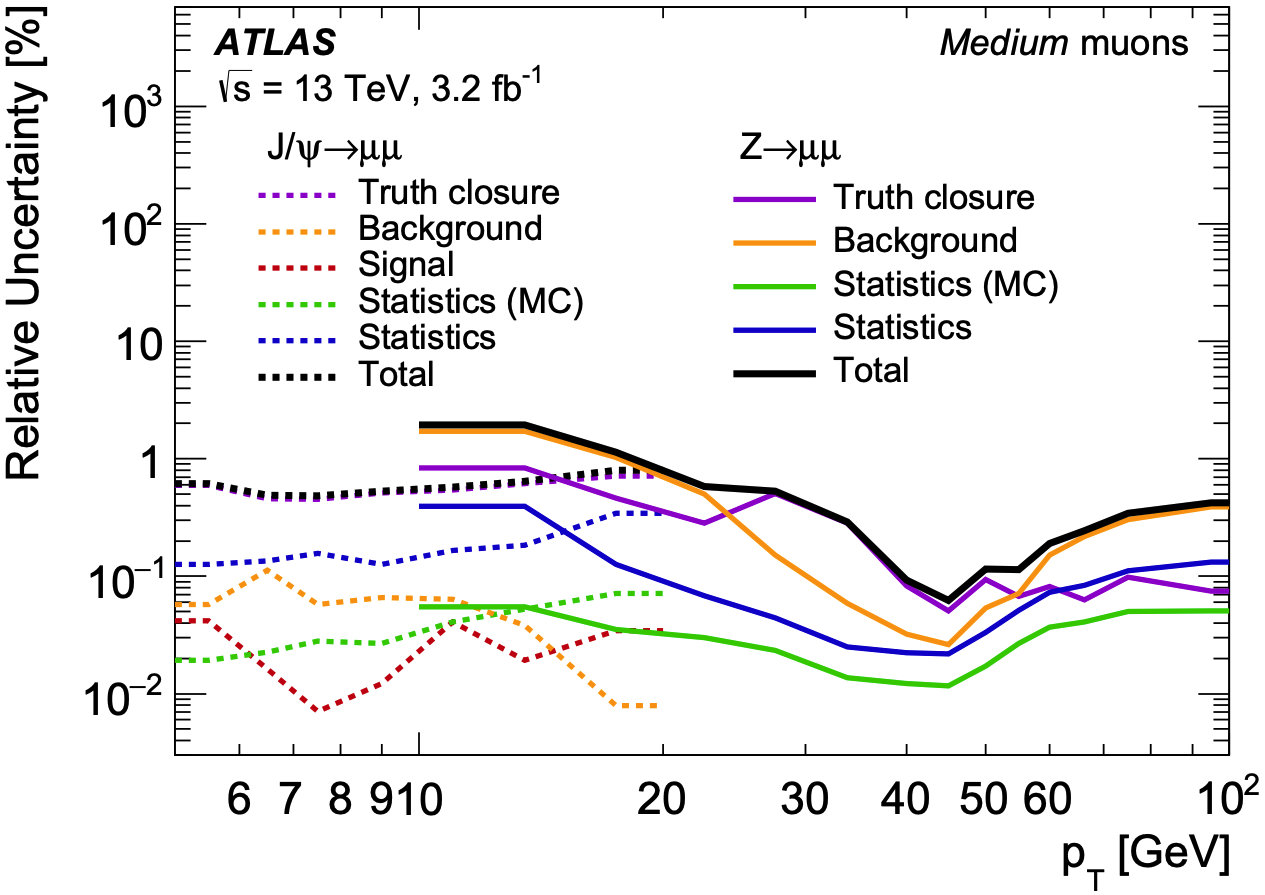
\includegraphics[width=0.8\linewidth]{figures/objects/medium_muons}
  \caption{\cite{Aad:2016jkr} Total uncertainty in the efficiency scale factor for Medium muons as a function of $p_{T}$ as obtained from $Z \rightarrow \mu\mu$ (solid lines) and $J/\Psi \rightarrow \mu\mu$ (dashed lines) decays. The combined uncertainty is the sum in quadrature of the individual contributions}
  \label{sec:objects:medium_muons}
\end{figure}
